\begin{align}
	\vec{m} &= \vec{A} - \vec{B}
= \myvec{-3\\5}
\implies
\vec{n} &= \myvec{5\\3}
\end{align}
Thus, the equation of line is
\begin{align}
 \myvec{ 5 & 3}\vec{x}  &= -2
\end{align}
See 
   \figref{fig:chapters/11/10/2/7/Line_AB}.
\begin{figure}[h!]
  \centering
   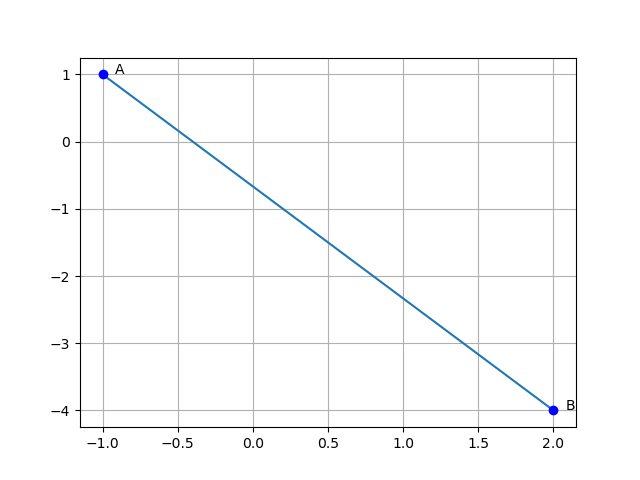
\includegraphics[width=\linewidth]{chapters/11/10/2/7/figs/Figure_1.png}
   \caption{}
   \label{fig:chapters/11/10/2/7/Line_AB}
\end{figure}




